\documentclass[a4paper,10pt]{article}
\usepackage[utf8]{inputenc}
\usepackage{amsmath}
\usepackage{graphicx}
\usepackage{hyperref}

\title{Exercise 1 Delivery: Constructive Analysis}
\author{Fellipe Pessanha}
\date{\today}

\begin{document}

\maketitle

\section{Exercise Description}
% Briefly describe what the first exercise was about.
The task in hand was to implement solution constructors for the specified software dependency
problem, in specific a \textit{random constructor}, \textit{randomized greedy constructor},
and a \textit{greedy constructor}, then perform a statistical analysis of their performance.


\section{Implementation Details}
% Explain how you approached and implemented the solution.
The implementation was carried out using \textbf{Julia}. The implementation steps involved
\begin{enumerate}
    \item Parsing the input data to extract problem context
    \item Implement a prototype evaluator in order to assess solution quality
    \item Write tests that make sure each step is working as expected
\end{enumerate}

The best way to understand the code structure is to check the~
\href{https://github.com/fellipessanha/postgrad-metaheuristics}{repository}'s test suite at
\texttt{./test/runtest.jl}

\subsection{Constructive implementation}

The randomized greedy constructive was implemented using a combination of a max heap $H$ --
keeping track of all the available packages sorted by their \textit{benefit} -- and a vector $V$
-- used to store all the $n$ best evaluated packages by the same criterion, guaranteeing
optimal $O(N \cdot log(\#H))$, where $N$ is the number of packages selected packages, and $\#H$
is the mean number of packages available in the unused heap throughout the execution.

The size of the vector is determined by the parameter $\alpha \in [0, 1]$, and the random
constructive was simply implemented by setting $\alpha = 1$, and the greedy constructive by
setting $\alpha = 0$.

\section{Analysis Methodology}

The analysis was performed for 30 equidistant values of $\alpha \in [0, 1]$.

In each step, 30 independent runs were performed for each constructor, and captured
the average solution quality, standard deviation, and execution time, evaluated with
Julia's \href{https://juliapackages.com/p/benchmarktools}{BenchmarkTools} package,
which accounts for garbage collection, precompilation time, and other Julia specific
nuances.

\section{Results}
% Present and discuss the results obtained.
The results of the analysis, normalized in \% values, can be seen in Figure~\ref{fig:results}.

\begin{figure}[!ht]
    \centering
    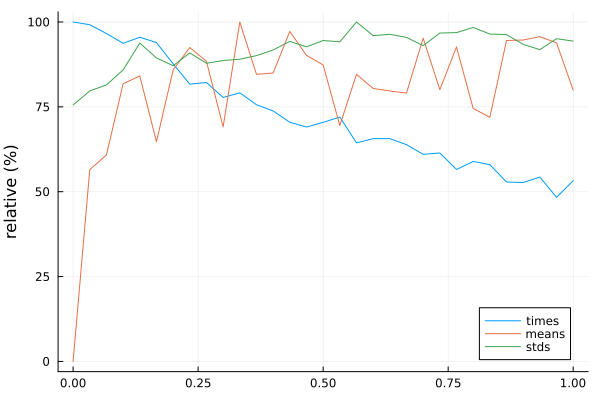
\includegraphics[width=0.7\textwidth]{../simple_constructive_analysis.png}
    \caption{mean solution quality, standard deviation, and time elapsed by $\alpha$}
    \label{fig:results}
\end{figure}

We can see in our plots that the execution time, aside from some noise and outliers, is mostly 
consistent during the entire range of $\alpha$ values, with a slight trend upwards as $\alpha$
increases. The standard deviation also seems mostly regular for $\alpha \in [0.1, 1]$, and the mean
value of the solutions consistently decreases as $\alpha$ increases, with the purely random
constructor ($\alpha = 1$) performing at about 50\% of the greedy constructor ($\alpha = 0$).

\section{Conclusion}
% Summarize your findings and any insights.

With the results in hand, we can conclude that, outside of a small range of small $\alpha$, our
constructor behaves consistently, having a standard deviation of a mostly random sample of values.

Knowing that $\alpha$ has very little impact on the execution time, we can also conclude that
the choice of $\alpha$ can be manipulated to achieve the desired balance of solution quality
and variety, and that values with $\alpha \in [0.3, 0.6]$ seem to be a good sweet spot.
\end{document}
